% CINEC Campus - Electronics Design Project Report Template
% Compile with: latexmk -pdf main.tex

\documentclass[12pt,a4paper,twoside,openany]{report}

% --- Encoding / language ---
\usepackage[T1]{fontenc}
\usepackage[utf8]{inputenc}
\usepackage[english]{babel}

% --- Page layout ---
% Binding-friendly margins (inner > outer)
\usepackage[a4paper,inner=1.5in,outer=1in,top=1in,bottom=1in]{geometry}
\usepackage{setspace}
\onehalfspacing

% --- Graphics / tables ---
\usepackage{graphicx}
\usepackage{float}
\usepackage{booktabs}
\usepackage{array}
\usepackage{multirow}

% --- LaTeX-only figures (optional) ---
\usepackage{tikz}
\usetikzlibrary{arrows.meta,positioning}

% --- Code listings (optional) ---
\usepackage{listings}
\usepackage{xcolor}
\lstset{
	basicstyle=\ttfamily\small,
	breaklines=true,
	frame=single,
	tabsize=2
}

% --- Math / units ---
\usepackage{amsmath}
\usepackage{amssymb}
\usepackage{siunitx}
\sisetup{detect-all}

% --- Links ---
\usepackage[hidelinks]{hyperref}

% Recommended with biblatex + babel
\usepackage{csquotes}

% --- Lists / TOC ---
\usepackage{tocloft}

% --- Headers / footers ---
\usepackage{fancyhdr}

% --- Bibliography ---
\usepackage[backend=biber,style=ieee]{biblatex}
\addbibresource{references.bib}

% --- Simple metadata macros (edit these) ---
\newcommand{\CampusName}{CINEC Campus}
\newcommand{\DepartmentName}{Department of Electrical and Electronic Engineering}
\newcommand{\ProgramName}{BSc. in Electronics and Telecommunication Engineering}
\newcommand{\ProjectTitle}{Design and Implementation of a \texorpdfstring{\\}{ }DC-DC Buck Converter for Embedded Systems}
\newcommand{\ProjectSubtitle}{Electronics Design Project Report}
\newcommand{\StudentName}{Your Name}
\newcommand{\StudentID}{Your Student ID}
\newcommand{\SupervisorName}{Supervisor Name}
\newcommand{\SubmissionDate}{\today}

% --- Header/footer styles ---
% Front matter: no header (page number only)
\fancypagestyle{frontmatter}{
	\fancyhf{}
	\fancyfoot[C]{\thepage}
	\renewcommand{\headrulewidth}{0pt}
	\renewcommand{\footrulewidth}{0pt}
}

% Main matter: chapter title in header, page number in footer
\setlength{\headheight}{15pt}
\fancypagestyle{mainmatter}{
	\fancyhf{}
	\fancyhead[L]{\small\nouppercase{\leftmark}}
	\fancyfoot[C]{\thepage}
	\renewcommand{\headrulewidth}{0.4pt}
	\renewcommand{\footrulewidth}{0pt}
}

\renewcommand{\chaptermark}[1]{\markboth{Chapter \thechapter: #1}{}}



\begin{document}

% --- Front matter ---
\pagenumbering{roman}
\pagestyle{frontmatter}
\begin{titlepage}
\begin{center}

% --- Logo (place file at figures/cinec-logo.png) ---
\IfFileExists{figures/cinec-logo.png}{%
	\includegraphics[width=0.55\textwidth]{figures/cinec-logo.png}\\[0.8cm]
}{}

{\Large \textbf{\CampusName}}\\[0.5cm]
{\DepartmentName}\\
{\ProgramName}\\[1.5cm]

{\LARGE \textbf{\ProjectTitle}}\\[0.4cm]
{\large \ProjectSubtitle}\\[1.5cm]

\begin{tabular}{@{}ll@{}}
\textbf{Student} & \StudentName \\
\textbf{Student ID} & \StudentID \\
\textbf{Supervisor} & \SupervisorName \\
\textbf{Date} & \SubmissionDate \\
\end{tabular}

\vfill

\textit{Submitted in partial fulfillment of the requirements for the Electronics Design Project.}

\end{center}
\end{titlepage}


\chapter*{Declaration}
\addcontentsline{toc}{chapter}{Declaration}

I declare that this report is my own work and has not been submitted in any form for another degree or diploma at any university or other institution of tertiary education.

All sources used have been acknowledged by means of complete references.

\vspace{1.5cm}

\noindent\textbf{Signature:} \rule{7cm}{0.4pt} \\
\textbf{Name:} \StudentName \\
\textbf{Date:} \SubmissionDate

\chapter*{Acknowledgements}
\addcontentsline{toc}{chapter}{Acknowledgements}

I would like to express my sincere gratitude to \SupervisorName for guidance throughout the electronics design process, and to the staff at \CampusName for providing the facilities and support required to complete this project.

I also thank my peers for their feedback during design reviews and testing sessions.

\chapter*{Abstract}
\addcontentsline{toc}{chapter}{Abstract}

This report presents the design, implementation, and testing of an electronics system developed as part of an Electronics Design Project at \CampusName. The sample project used in this template is a \SI{12}{\volt} to \SI{5}{\volt} synchronous buck converter intended for embedded systems.

The report covers requirements definition, circuit selection, component calculations, PCB considerations, firmware (if applicable), verification tests, and measured results. The template is structured to support typical electronics deliverables including a block diagram, schematic references, bill of materials (BOM), test plan, and compliance considerations.


\chapter*{Abbreviations}
\addcontentsline{toc}{chapter}{Abbreviations}

\begin{tabular}{@{}ll@{}}
\textbf{BOM} & Bill of Materials \\
\textbf{DC} & Direct Current \\
\textbf{DRC} & Design Rule Check \\
\textbf{EMI} & Electromagnetic Interference \\
\textbf{ESD} & Electrostatic Discharge \\
\textbf{MCU} & Microcontroller \\
\textbf{PCB} & Printed Circuit Board \\
\textbf{PSU} & Power Supply Unit \\
\end{tabular}


\newpage
\tableofcontents

\newpage
\listoffigures

\newpage
\listoftables

\clearpage
\pagenumbering{arabic}

% From here on, use chapter header style
\pagestyle{mainmatter}
\fancypagestyle{plain}{
	\fancyhf{}
	\fancyfoot[C]{\thepage}
	\renewcommand{\headrulewidth}{0pt}
	\renewcommand{\footrulewidth}{0pt}
}

% --- Main content ---
\chapter{Introduction}

\section{Background}
Electronics design projects commonly require translating a set of system-level constraints (input supply range, output regulation, efficiency, thermal limits, cost, and manufacturability) into an implementable circuit and testable prototype. Standard circuit design references and vendor application notes are commonly used to justify design choices and calculations \cite{sedra_smith_microelectronic_2014,ti_buck_design}.

\section{Project Overview}
This template assumes an example power electronics subsystem: a regulated \SI{5}{\volt} rail derived from a \SI{12}{\volt} source for a microcontroller-based embedded system.

\section{Objectives}
\begin{itemize}
  \item Define measurable electrical and mechanical requirements.
  \item Design and simulate the circuit (where applicable).
  \item Implement the design on a PCB and assemble a prototype.
  \item Verify performance using a documented test plan.
\end{itemize}

\section{Report Structure}
Chapter 2 defines requirements, Chapters 3--4 describe design and implementation, Chapters 5--6 present verification and results, and the final chapter summarizes conclusions and future work.

\chapter{Requirements Specification}

\section{Functional Requirements}
\begin{itemize}
  \item Convert input voltage to a regulated \SI{5}{\volt} output.
  \item Provide load current up to \SI{2}{\ampere}.
  \item Maintain output ripple below \SI{50}{\milli\volt_{pp}} under nominal conditions.
\end{itemize}

\section{Non-Functional Requirements}
\begin{itemize}
  \item Efficiency $\ge 85\%$ at \SI{1}{\ampere} load.
  \item Thermal: keep hottest component case temperature below \SI{85}{\celsius} in still air.
  \item PCB: 2-layer FR4, standard fabrication constraints (track/space, via sizes).
\end{itemize}

\section{Constraints and Assumptions}
\begin{itemize}
  \item Input supply: \SI{10}{\volt} to \SI{14}{\volt}.
  \item Ambient temperature: \SI{25}{\celsius} (unless otherwise stated).
  \item Measurement equipment: oscilloscope, electronic load, DMM.
\end{itemize}

\section{Acceptance Criteria}
Table~\ref{tab:acceptance} summarizes the acceptance criteria.

\begin{table}[H]
  \centering
  \caption{Acceptance criteria}
  \label{tab:acceptance}
  % LaTeX-only sample table include
% Use inside a table environment: % LaTeX-only sample table include
% Use inside a table environment: \input{tables/acceptance_criteria}

\begin{tabular}{@{}lll@{}}
  \toprule
  \textbf{Metric} & \textbf{Target} & \textbf{Test method} \\
  \midrule
  Output voltage & \SI{5.0}{\volt} \,$\pm$\,\SI{3}{\percent} & DMM at load \\
  Output ripple & $<\SI{50}{\milli\volt_{pp}}$ & Oscilloscope AC-coupled \\
  Efficiency & $\ge 85\%$ @ \SI{1}{\ampere} & Power in/out \\
  Temperature & $<\SI{85}{\celsius}$ & Thermocouple/IR \\
  \bottomrule
\end{tabular}


\begin{tabular}{@{}lll@{}}
  \toprule
  \textbf{Metric} & \textbf{Target} & \textbf{Test method} \\
  \midrule
  Output voltage & \SI{5.0}{\volt} \,$\pm$\,\SI{3}{\percent} & DMM at load \\
  Output ripple & $<\SI{50}{\milli\volt_{pp}}$ & Oscilloscope AC-coupled \\
  Efficiency & $\ge 85\%$ @ \SI{1}{\ampere} & Power in/out \\
  Temperature & $<\SI{85}{\celsius}$ & Thermocouple/IR \\
  \bottomrule
\end{tabular}

\end{table}

\chapter{Design}

\section{System Block Diagram}
Figure~\ref{fig:block} shows a typical block-level decomposition.

\begin{figure}[H]
  \centering
  % LaTeX-only sample figure (TikZ)
% Use inside a figure environment: % LaTeX-only sample figure (TikZ)
% Use inside a figure environment: \input{figures/block_diagram}

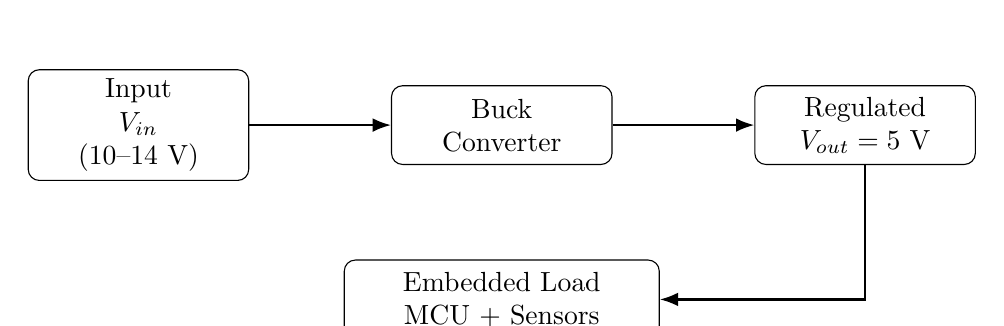
\begin{tikzpicture}[
  block/.style={draw, rounded corners, align=center, minimum height=10mm, minimum width=28mm},
  arrow/.style={-Latex, thick}
]

\node[block] (vin) {Input\\$V_{in}$\\(10--14 V)};
\node[block, right=18mm of vin] (buck) {Buck\\Converter};
\node[block, right=18mm of buck] (vout) {Regulated\\$V_{out}=5$ V};
\node[block, below=12mm of buck, minimum width=40mm] (load) {Embedded Load\\MCU + Sensors};

\draw[arrow] (vin) -- (buck);
\draw[arrow] (buck) -- (vout);
\draw[arrow] (vout) |- (load);

\end{tikzpicture}


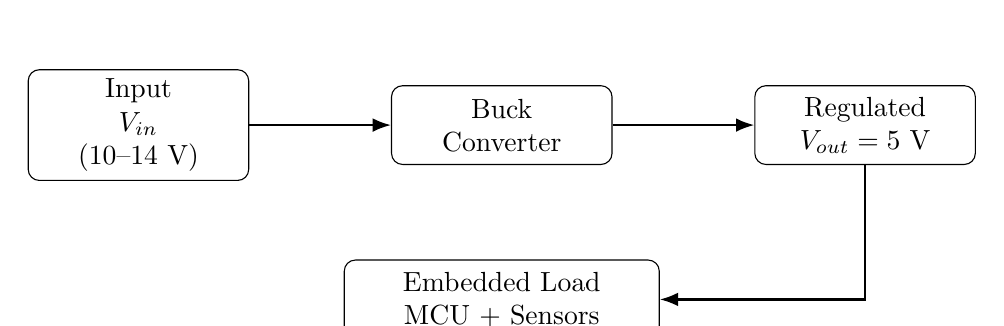
\begin{tikzpicture}[
  block/.style={draw, rounded corners, align=center, minimum height=10mm, minimum width=28mm},
  arrow/.style={-Latex, thick}
]

\node[block] (vin) {Input\\$V_{in}$\\(10--14 V)};
\node[block, right=18mm of vin] (buck) {Buck\\Converter};
\node[block, right=18mm of buck] (vout) {Regulated\\$V_{out}=5$ V};
\node[block, below=12mm of buck, minimum width=40mm] (load) {Embedded Load\\MCU + Sensors};

\draw[arrow] (vin) -- (buck);
\draw[arrow] (buck) -- (vout);
\draw[arrow] (vout) |- (load);

\end{tikzpicture}

  \caption{System block diagram (LaTeX-only sample)}
  \label{fig:block}
\end{figure}

\section{Topology Selection}
A buck converter is appropriate when stepping down a higher DC input voltage to a lower DC output voltage with high efficiency \cite{ti_buck_design}.

\section{Key Design Calculations (Example)}
For an ideal buck converter, the duty cycle is approximately:
\begin{equation}
  D \approx \frac{V_{out}}{V_{in}}
\end{equation}

Assuming $V_{in}=\SI{12}{\volt}$ and $V_{out}=\SI{5}{\volt}$, then:
\begin{equation}
  D \approx \frac{5}{12} \approx 0.417
\end{equation}

\section{Component Selection}
Document IC selection rationale (availability, features, protection, switching frequency).

\subsection{Bill of Materials (Excerpt)}
\begin{table}[H]
  \centering
  \caption{BOM excerpt (example format)}
  \label{tab:bom}
  % LaTeX-only sample table include
% Use inside a table environment: % LaTeX-only sample table include
% Use inside a table environment: \input{tables/bom_excerpt}

\begin{tabular}{@{}llll@{}}
  \toprule
  \textbf{RefDes} & \textbf{Value/Part} & \textbf{Package} & \textbf{Notes} \\
  \midrule
  U1 & Buck Regulator IC & QFN & Synchronous, \SI{500}{\kilo\hertz} \\
  L1 & \SI{4.7}{\micro\henry} & SMD & Saturation current $>\SI{3}{\ampere}$ \\
  COUT & 2 $\times$ \SI{22}{\micro\farad} & 1206 & Low-ESR ceramic \\
  \bottomrule
\end{tabular}


\begin{tabular}{@{}llll@{}}
  \toprule
  \textbf{RefDes} & \textbf{Value/Part} & \textbf{Package} & \textbf{Notes} \\
  \midrule
  U1 & Buck Regulator IC & QFN & Synchronous, \SI{500}{\kilo\hertz} \\
  L1 & \SI{4.7}{\micro\henry} & SMD & Saturation current $>\SI{3}{\ampere}$ \\
  COUT & 2 $\times$ \SI{22}{\micro\farad} & 1206 & Low-ESR ceramic \\
  \bottomrule
\end{tabular}

\end{table}

\section{PCB Design Considerations}
Include placement rules, high-current loop minimization, ground strategy, and thermal vias. Reference your layout screenshots or 3D render exports. Thermal performance and copper utilization should be justified with appropriate references when relevant \cite{ieee_thermal_pcb}.

\chapter{Implementation}

\section{Schematic Capture}
Provide a short description of the schematic organization (power stage, feedback network, protection, connectors). Include figure exports as needed.

\section{PCB Layout}
Include:
\begin{itemize}
  \item Layer stack-up (2-layer example)
  \item Critical nets and current paths
  \item Design rule checks (DRC)
\end{itemize}

\section{Prototype Assembly}
Document the assembly process, tools used, and any rework performed.

\section{Firmware (If Applicable)}
If the design includes firmware (e.g., telemetry, fault logging), describe:
\begin{itemize}
  \item Architecture and modules
  \item Interfaces (I\textsuperscript{2}C, SPI, UART)
  \item Key parameters and calibration
\end{itemize}

\chapter{Testing and Verification}

\section{Test Setup}
Describe the measurement setup, including power supply, load, oscilloscope probe method (tip-and-barrel spring), and grounding. Use vendor guidance and best practices for switching regulator measurement where applicable \cite{ti_buck_design}.

\section{Test Plan}
\begin{table}[H]
  \centering
  \caption{Test plan summary}
  \label{tab:testplan}
  \begin{tabular}{@{}llll@{}}
    \toprule
    \textbf{Test ID} & \textbf{Condition} & \textbf{Measurement} & \textbf{Expected} \\
    \midrule
    T1 & $V_{in}=\SI{12}{\volt}$, $I_{out}=\SI{0.5}{\ampere}$ & $V_{out}$ & \SI{5}{\volt} \,$\pm$\,\SI{3}{\percent} \\
    T2 & $V_{in}=\SI{12}{\volt}$, $I_{out}=\SI{2}{\ampere}$ & Ripple & $<\SI{50}{\milli\volt_{pp}}$ \\
    T3 & Sweep load 0--\SI{2}{\ampere} & Efficiency & $\ge 85\%$ @ \SI{1}{\ampere} \\
    T4 & \SI{25}{\celsius} ambient & Hotspot temp & $<\SI{85}{\celsius}$ \\
    \bottomrule
  \end{tabular}
\end{table}

\section{Safety and Handling}
Include ESD precautions, current limit settings, and safe probing practices.

\chapter{Results and Discussion}

\section{Measured Performance}
Summarize key measurements in a table.

\begin{table}[H]
  \centering
  \caption{Measured results (example placeholders)}
  \label{tab:results}
  \begin{tabular}{@{}lll@{}}
    \toprule
    \textbf{Metric} & \textbf{Measured} & \textbf{Notes} \\
    \midrule
    Output voltage @ \SI{1}{\ampere} & \SI{5.02}{\volt} & Within tolerance \\
    Ripple @ \SI{2}{\ampere} & \SI{38}{\milli\volt_{pp}} & Tip-and-barrel method \\
    Efficiency @ \SI{1}{\ampere} & 88\% & \SI{12}{\volt} input \\
    Max hotspot temperature & \SI{72}{\celsius} & Still air, 10 min \\
    \bottomrule
  \end{tabular}
\end{table}

\section{Discussion}
Discuss deviations from expected results, sources of error, and improvements (layout changes, component derating, compensation tuning).

\section{Comparison to Requirements}
Reference Table~\ref{tab:acceptance} and explicitly state pass/fail for each criterion.

\chapter{Conclusion and Future Work}

\section{Conclusion}
This project demonstrated an end-to-end electronics design workflow: requirements definition, circuit design, PCB implementation, and verification against measurable acceptance criteria.

\section{Future Work}
\begin{itemize}
  \item Extend the input range and add surge protection.
  \item Improve thermal performance using copper pours and additional vias.
  \item Add output telemetry and fault logging.
\end{itemize}


% --- References ---
\clearpage
\printbibliography

% --- Appendices ---
\appendix
\chapter{Appendix A: Additional Materials}

\section{Datasheets and Design Notes}
Include links and notes used during the design.

\section{Schematic / PCB Exports}
Place exported PDFs/PNGs in the \texttt{figures/} folder and reference them from the relevant chapters.

\section{Example Figure Include}
\begin{figure}[H]
  \centering
  % Example: \includegraphics[width=0.9\textwidth]{figures/pcb-top.pdf}
  \fbox{\parbox{0.85\textwidth}{\centering Placeholder: PCB top layer (export to figures/pcb-top.pdf)}}
  \caption{PCB top layer (placeholder)}
\end{figure}


\end{document}
